% =====================================================================
% Missingness-Aware Transformer for Air-Quality Forecasting
% Default class: elsarticle (applied/environmental venues; e.g. Expert
% Systems with Applications, Environmental Modelling & Software).
% To retarget an IEEE venue, swap the class for IEEEtran and remove the
% elsarticle front-matter macros.
% Build:  latexmk -pdf main.tex     (or pdflatex x2 + bibtex)
% Figures/tables are produced by scripts/07_make_paper_assets.py.
% =====================================================================
\documentclass[review,3p,times]{elsarticle}

\usepackage[utf8]{inputenc}
\usepackage{amsmath,amssymb}
\usepackage{graphicx}
\usepackage{booktabs}
\usepackage{siunitx}
\usepackage{multirow}
\usepackage{xcolor}
\usepackage[hidelinks]{hyperref}
\usepackage{microtype}

\graphicspath{{../outputs/figures/}{../outputs/beijing/figures/}}
\sisetup{detect-weight=true, detect-family=true}
\newcommand{\ugm}{\si{\micro\gram\per\cubic\metre}}
\newcommand{\pmf}{PM\textsubscript{2.5}}

\journal{Expert Systems with Applications}

\begin{document}

\begin{frontmatter}

\title{When to Forecast End-to-End versus Impute-then-Forecast:
A Missingness-Severity Crossover for Air-Quality Prediction on
Incomplete Monitoring Networks}

\author[a]{Anonymous Author}
\address[a]{Anonymous Institution}

\begin{abstract}
Operational air-quality monitoring networks produce severely incomplete
multivariate streams, yet the prevailing practice is a two-stage
\emph{impute-then-forecast} pipeline whose imputation stage must be refit and
re-run on every data refresh. We ask a question that the literature has left
implicit: \emph{when} should one forecast end-to-end from masked inputs rather
than impute first? We answer it with a controlled study on two monitoring
networks of very different completeness---Dhaka, Bangladesh (\pmf{} \SI{23.4}{\percent}
missing) and the Beijing Multi-Site benchmark (\SI{2.1}{\percent} missing)---using a
deliberately simple, CPU-deployable missingness-aware Transformer that consumes
the observation mask natively. Against strong baselines including the
missingness-native GRU-D recurrent model and three impute-then-forecast
pipelines (KNN, MICE, and the deep self-attention imputer SAITS), the end-to-end
model reaches \emph{accuracy parity} at every horizon on both networks; per-seed
Diebold--Mariano tests confirm no significant difference, correcting a
single-seed result in earlier work that did not replicate. The central finding
is a \emph{missingness-severity crossover governed by two factors}, not one.
On the severely incomplete, less-structured Dhaka network the advantage of
end-to-end forecasting over even a deep imputer rises with input incompleteness:
stratifying natural test windows by completeness, end-to-end trails the deep
imputer by \SI{2.1}{\ugm} on the most complete windows but leads by \SI{2.3}{\ugm}
on the most incomplete, and under synthetic station outages it overtakes above
$\approx\!38\%$ effective input missingness at \SI{6}{\hour}. This threshold is
\emph{not} universal: on the highly periodic Beijing network a deep imputer
remains best under outages at every tested severity---its margin even grows---
because strong diurnal structure keeps large outage blocks imputable. Under
cell-wise MCAR a deep imputer wins on both networks. The practical rule is thus
conditional on both missingness severity and series imputability: end-to-end
forecasting (with training-time missingness dropout, which also wins on
high-pollution episodes) is preferable in the high-missingness, low-imputability
regime; impute-then-forecast wins otherwise. We
provide the crossover as a deployment decision rule, a fully reproducible
multi-seed benchmark, and a data-quality lesson on sensor error codes that, left
unhandled, distort every reported number.
\end{abstract}

\begin{keyword}
air quality forecasting \sep missing data \sep transformer \sep
time series imputation \sep \pmf{} \sep deployable machine learning
\end{keyword}

\end{frontmatter}

% =====================================================================
\section{Introduction}
\label{sec:intro}

Fine particulate matter (\pmf) is among the largest environmental risk factors
for human health \citep{who2021guidelines,kim2009review}, and short-horizon
\pmf{} forecasts drive public advisories and exposure mitigation. The data that
must feed those forecasts, however, are produced by physical monitoring networks
that are routinely and severely incomplete: sensors fail, stations go offline
for days, and entire variables are absent at some sites. In our Dhaka network,
\pmf{} is \SI{23.4}{\percent} missing overall (\SIrange{10}{45}{\percent} per
station), and roughly \SI{39}{\percent} of missing \pmf{} hours fall in gaps
longer than seven days---missingness is dominated by structured \emph{station
outages}, not independent dropout.

The dominant response in the forecasting literature is the \emph{two-stage} or
\emph{impute-then-forecast} pipeline: first reconstruct a complete series with a
statistical or deep imputer, then forecast from the completed series. This is
operationally costly---the imputer is part of the serving path and must be refit
and re-run whenever new data arrive---and it presumes that imputation is
reliable. An alternative is to forecast \emph{end-to-end} from the incomplete
series, letting the model consume the observation mask directly
\citep{che2018grud}. Which paradigm should a practitioner deploy?

The literature largely argues this implicitly, by reporting aggregate accuracy
of one method against another on a single dataset. We argue that the honest and
useful question is conditional: the right paradigm depends on \emph{how much} and
\emph{what kind of} missingness the deployment faces. We make this concrete by
characterizing the \textbf{missingness-severity crossover}---the effective
input-missingness level at which end-to-end forecasting overtakes
impute-then-forecast---across two networks that bracket the severity spectrum and
a controlled corruption sweep that holds the dataset fixed.

Our contributions are:
\begin{enumerate}
  \item A \textbf{controlled characterization of when end-to-end forecasting
  beats impute-then-forecast}, showing the choice is governed by the interaction
  of effective input missingness, missingness structure (cell-wise vs
  station-outage), and series imputability---yielding a conditional deployment
  decision rule and a clean within-network crossover on severely incomplete data
  (Section~\ref{sec:crossover}).
  \item A \textbf{simple, CPU-deployable missingness-aware Transformer} that
  reaches accuracy parity with strong impute-then-forecast pipelines---including
  a quality-gated deep imputer (SAITS)---and the missingness-native GRU-D, on two
  networks, while eliminating the imputation stage
  (Sections~\ref{sec:method}--\ref{sec:results}).
  \item \textbf{Training-time missingness dropout}, which buys the strongest
  robustness in the severe regime and the best high-pollution-episode accuracy,
  at a cost of $\approx$\SI{0.5}{\ugm} of clean accuracy.
  \item A \textbf{fully reproducible multi-seed benchmark} (three seeds,
  per-seed Diebold--Mariano significance, deterministic pipeline, 86 tests) and a
  reusable \textbf{data-quality lesson}: undocumented sensor saturation codes
  that, if not removed, inflate even a persistence baseline by \SI{40}{\ugm}.
\end{enumerate}

We are explicit about the limits of the contribution. The architecture is
deliberately conventional; the novelty is the crossover characterization and the
deployability argument, not a new accuracy state of the art. Where a baseline
wins---SAITS under cell-wise MCAR on both networks, and under station outages on
the near-complete Beijing network---we report it.

% =====================================================================
\section{Related work}
\label{sec:related}

\paragraph{Learning from incomplete time series.}
GRU-D \citep{che2018grud} is the canonical missingness-native recurrent model,
introducing learned input- and hidden-state decay driven by the time since last
observation; we implement it faithfully as a baseline. BRITS \citep{cao2018brits}
casts imputation as bidirectional recurrent estimation. Attention-based models
for irregular and missing series include mTAND \citep{shukla2021mtan}, which
learns continuous-time attention, and Raindrop \citep{zhang2022raindrop}, which
models sensor dependencies as a graph. Our model sits at the simple end of this
spectrum by design: a standard pre-norm Transformer encoder with a learned
missingness embedding and optional mask-restricted attention, chosen for
CPU-deployability rather than architectural novelty.

\paragraph{Imputation and impute-then-forecast.}
Classical imputers---$k$-nearest-neighbours \citep{troyanskaya2001missing} and
multivariate imputation by chained equations
(MICE)~\citep{vanbuuren2011mice}---remain standard practice
\citep{moritz2017imputets}, grounded in the missing-data theory of
\citet{little2019statistical}. Deep imputers have advanced quickly: SAITS
\citep{du2023saits} uses diagonally-masked self-attention with a joint
reconstruction objective, and CSDI \citep{tashiro2021csdi} uses conditional
diffusion. We include SAITS as a \emph{strong} impute-then-forecast competitor,
quality-gated so that it genuinely outperforms forward-fill before it is used.
Crucially, prior work compares end-to-end and impute-then-forecast methods at a
single operating point; we instead trace the comparison across the missingness
spectrum and locate the crossover.

\paragraph{Time-series forecasting architectures.}
Recent general forecasters include DLinear \citep{zeng2023dlinear}, which shows a
simple linear model is a strong baseline, and PatchTST \citep{nie2023patchtst},
a channel-independent patching Transformer; both are included. Long-horizon
Transformers such as Autoformer \citep{wu2021autoformer} and Pyraformer
\citep{liu2022pyraformer} target a different (clean, long-context) regime.
Spatiotemporal air-quality models such as GeoMAN \citep{liang2018geoman} exploit
network geometry; we keep a per-station treatment to isolate the effect of
missingness handling.

% =====================================================================
\section{Data and missingness characterization}
\label{sec:data}

\paragraph{Networks.}
We use two hourly air-quality networks. \textbf{Dhaka} comprises 16 monitoring
stations across Bangladesh (2022--2024), with six target pollutants (\pmf, PM10,
NO\textsubscript{2}, O\textsubscript{3}, CO, SO\textsubscript{2}) and
meteorology. \textbf{Beijing Multi-Site} \citep{zhang2017cautionary} comprises 12
stations (2013--2017) with the same six pollutants and meteorology. The two
bracket the missingness spectrum: Dhaka \pmf{} is \SI{23.4}{\percent} missing,
Beijing only \SI{2.1}{\percent}.

\paragraph{Missingness is structured and not at random.}
On Dhaka, a logistic regression predicting the \pmf{} missingness indicator from
observed meteorology and calendar features attains held-out AUC $0.606$, ruling
out missing-completely-at-random; pollutant missingness indicators are correlated
($\bar{r}\approx0.38$), consistent with station-level outages. This motivates two
synthetic corruption mechanisms in our robustness study
(Section~\ref{sec:robustness}): cell-wise MCAR (an easy case that preserves each
timestep's cross-section) and station-outage blocks (\SIrange{6}{48}{\hour}
all-variable gaps, matching the dominant real mechanism).

\paragraph{Data-quality lesson.}
The 2024 Dhaka files contain sensor saturation/error codes (the value
\num{985.0} repeats verbatim thousands of times, including in monsoon months
where such concentrations are physically impossible). Treating these as
measurements inflates the persistence \SI{6}{\hour} RMSE from \SI{94}{} to
\SI{134}{\ugm}; every model comparison would be distorted. We flag-and-remove
such codes and document the full cleaning protocol. Table~\ref{tab:dataset}
(\texttt{table1\_dataset\_summary}) summarizes per-station coverage.

% =====================================================================
\section{Method}
\label{sec:method}

\paragraph{Inputs and masks.}
For each station we form windows of $L=168$ input hours and predict horizons
$\{6,24,72\}$ for all six targets. Each window carries scaled values
$x\in\mathbb{R}^{L\times V}$ (missing cells set to zero), an observation mask
$m\in\{0,1\}^{L\times V}$, cyclic calendar features, and a station id. Scalers
are fit on the training period only.

\paragraph{Missingness-aware Transformer.}
The encoder input is
\begin{equation}
h = W_v x + \mathbf{1}[\text{embed}]\,W_m(\mathbf{1}-m) + W_t \text{cal} + e_{\text{station}} + \text{PE},
\end{equation}
where $W_m(\mathbf{1}-m)$ is a learned per-variable \emph{missingness embedding}
so that ``absent'' is distinguishable from ``measured zero.'' A standard pre-norm
Transformer encoder \citep{vaswani2017attention} (3 layers,
$d_{\text{model}}=128$, 8 heads, FFN 256) is followed by a per-horizon linear
head producing $(T,H)$ predictions. An optional
\emph{variant B} additionally masks attention to timesteps where the primary
target is unobserved. The model has \num{406418} parameters and runs at
\SI{1.8}{\milli\second} per window on a desktop CPU. Training minimizes a masked
mean-squared error over observed targets only.

\paragraph{Missingness dropout.}
To harden the model against missingness levels beyond those seen in training, we
optionally apply \emph{missingness dropout}: during training a random fraction
$U[0,0.5]$ of observed input cells is additionally masked each step. This is the
only difference between ``Proposed'' and ``Proposed + miss-dropout.''

\paragraph{Impute-then-forecast baselines.}
For a controlled comparison, the two-stage pipelines use a \emph{size-identical}
vanilla Transformer (same architecture without the missingness pathway) on
inputs completed by KNN \citep{troyanskaya2001missing}, MICE
\citep{vanbuuren2011mice}, or SAITS \citep{du2023saits}. Imputers are fit on
training rows only. Our SAITS implementation follows the original
diagonally-masked self-attention with a joint observed-reconstruction (ORT) and
masked-imputation (MIT) objective; before use we \emph{gate} it, requiring its
held-out reconstruction MAE to beat forward-fill (it does: $0.170$ vs $0.192$).

\paragraph{Additional baselines.}
We further include GRU-D \citep{che2018grud}, LSTM/GRU on forward-filled inputs,
DLinear \citep{zeng2023dlinear}, PatchTST \citep{nie2023patchtst} on
mask-concatenated inputs, and persistence, seasonal-naive, and per-station SARIMA.

% =====================================================================
\section{Experimental setup}
\label{sec:setup}

Splits are strictly chronological with the final year held out as test
(no window crosses a split boundary through its targets). Every learned model is
trained with three seeds (42/43/44); we report mean~$\pm$~std. Statistical
baselines are deterministic single runs. Significance uses a \emph{per-seed}
Diebold--Mariano test \citep{diebold1995comparing} with the small-sample
correction of \citet{harvey1997testing} and a paired bootstrap, pairing the
proposed model's seed~$i$ against the baseline's seed~$i$; we report the median
and range of $p$ across seeds. We deliberately do not average predictions across
seeds before testing, as that would evaluate a three-member ensemble that is
never deployed. Optimization is AdamW \citep{loshchilov2019adamw} with cosine
decay and early stopping. Metrics are RMSE (headline), MAE, and $R^2$, all
unscaled over observed targets; we additionally report a high-pollution-episode
RMSE restricted to test hours with observed \pmf{}~$>\SI{150}{\ugm}$. The
pipeline is config-driven and deterministic; all numbers regenerate from one
command, and 86 unit tests cover the contracts.

% =====================================================================
\section{Results}
\label{sec:results}

\subsection{Accuracy parity on both networks}
\label{sec:parity}

Table~\ref{tab:main} reports \pmf{} RMSE on Dhaka. The proposed model, variant B,
and the three two-stage pipelines (KNN, MICE, SAITS) lie within each other's
$\pm$std at every horizon. Per-seed Diebold--Mariano finds \emph{no significant
difference} between the proposed model and any of LSTM, GRU, GRU-D, KNN, MICE, or
SAITS at any horizon. Notably, a previously reported result---``two-stage KNN
significantly better at \SI{24}{\hour} ($p=0.042$)''---was a single-seed
artifact: across seeds $p = 0.038/0.042/0.891$ with a mean RMSE difference of
\SI{+0.04}{\ugm}. Variant~B is significantly better than the plain proposed model
at \SI{72}{\hour} (all seeds, median $p=0.006$), and the proposed family is
significantly better than DLinear and PatchTST everywhere. The same parity holds
on Beijing (Table~\ref{tab:beijing}), where the proposed model and variant~B are
in fact marginally the best at \SI{6}{\hour}.

\begin{table}[t]
\centering
\caption{Dhaka \pmf{} test RMSE (\ugm), three-seed mean~$\pm$~std for learned
models. Statistical baselines are deterministic. Best per column in bold.}
\label{tab:main}
\small
\begin{tabular}{lccc}
\toprule
Model & \SI{6}{\hour} & \SI{24}{\hour} & \SI{72}{\hour} \\
\midrule
Persistence            & 93.90 & 99.02 & 105.13 \\
Seasonal-naive         & 90.59 & 93.67 & 102.18 \\
SARIMA                 & 79.96 & 83.87 & 86.74 \\
LSTM                   & 68.20\,$\pm$\,0.34 & 78.05\,$\pm$\,0.08 & 80.95\,$\pm$\,0.79 \\
GRU                    & 67.69\,$\pm$\,0.47 & 76.45\,$\pm$\,0.20 & \textbf{79.58\,$\pm$\,0.37} \\
GRU-D                  & 68.89\,$\pm$\,0.31 & 76.69\,$\pm$\,0.49 & 80.61\,$\pm$\,0.24 \\
DLinear                & 70.51\,$\pm$\,0.72 & 80.90\,$\pm$\,1.34 & 83.55\,$\pm$\,0.40 \\
PatchTST               & 74.61\,$\pm$\,1.07 & 84.34\,$\pm$\,1.14 & 87.51\,$\pm$\,1.34 \\
Two-stage (KNN)        & \textbf{66.95\,$\pm$\,0.58} & 76.42\,$\pm$\,0.75 & 80.95\,$\pm$\,1.52 \\
Two-stage (MICE)       & 67.39\,$\pm$\,0.25 & 76.81\,$\pm$\,0.68 & 80.66\,$\pm$\,1.13 \\
Two-stage (SAITS)      & 67.22\,$\pm$\,0.82 & 76.31\,$\pm$\,0.40 & 81.43\,$\pm$\,1.15 \\
Proposed (MAT)         & 67.03\,$\pm$\,0.28 & 76.46\,$\pm$\,0.51 & 81.54\,$\pm$\,1.29 \\
Proposed (variant B)   & 67.04\,$\pm$\,0.29 & \textbf{76.00\,$\pm$\,0.51} & 80.26\,$\pm$\,1.36 \\
Proposed + miss-dropout& 67.48\,$\pm$\,0.88 & 79.69\,$\pm$\,1.77 & 81.54\,$\pm$\,0.91 \\
\bottomrule
\end{tabular}
\end{table}

\begin{table}[t]
\centering
\caption{Beijing Multi-Site \pmf{} test RMSE (\ugm), three-seed mean~$\pm$~std.
GPU-trained; accuracy parity holds, with the proposed family marginally best at
\SI{6}{\hour}.}
\label{tab:beijing}
\small
\begin{tabular}{lccc}
\toprule
Model & \SI{6}{\hour} & \SI{24}{\hour} & \SI{72}{\hour} \\
\midrule
GRU                    & 51.44\,$\pm$\,0.63 & 75.90\,$\pm$\,0.18 & 84.88\,$\pm$\,0.37 \\
GRU-D                  & 50.15\,$\pm$\,0.12 & \textbf{75.87\,$\pm$\,0.48} & 84.77\,$\pm$\,0.37 \\
DLinear                & 51.55\,$\pm$\,0.70 & 80.62\,$\pm$\,0.33 & 89.94\,$\pm$\,0.19 \\
PatchTST               & 58.50\,$\pm$\,0.73 & 79.71\,$\pm$\,0.89 & 87.54\,$\pm$\,1.59 \\
Two-stage (KNN)        & 49.67\,$\pm$\,0.66 & 76.83\,$\pm$\,0.37 & 86.78\,$\pm$\,0.99 \\
Two-stage (SAITS)      & 50.28\,$\pm$\,0.77 & 76.61\,$\pm$\,0.40 & 87.72\,$\pm$\,1.46 \\
Proposed (MAT)         & 49.43\,$\pm$\,0.72 & 76.79\,$\pm$\,0.36 & \textbf{86.37\,$\pm$\,0.45} \\
Proposed (variant B)   & \textbf{49.38\,$\pm$\,0.74} & 76.74\,$\pm$\,0.29 & 86.46\,$\pm$\,0.70 \\
Proposed + miss-dropout& 51.44\,$\pm$\,0.61 & 76.37\,$\pm$\,0.25 & 85.58\,$\pm$\,0.24 \\
\bottomrule
\end{tabular}
\end{table}

\subsection{Robustness under corruption}
\label{sec:robustness}

Figure~\ref{fig:robustness} traces \pmf{} RMSE as we inject additional cell-wise
MCAR and station-outage missingness into the Dhaka test inputs. Two facts stand
out at the operationally critical \SI{6}{\hour} horizon. Under MCAR, two-stage
SAITS is essentially flat (slope \SI{+0.0}{\ugm} at $+50\%$): the deep imputer
reconstructs the intact cross-section almost perfectly, and the plain proposed
model degrades fastest (\SI{+5.9}{\ugm}). Under station outages, the ordering
reverses: \emph{missingness dropout} has the flattest slope (\SI{+2.0}{\ugm}) and
the lowest RMSE at $+50\%$, ahead of SAITS (\SI{+3.9}{\ugm}) and KNN
(\SI{+3.5}{\ugm}). PatchTST and DLinear collapse under both. The mechanism is
intuitive: when a whole station block is missing, a row-wise or attention imputer
has no contemporaneous signal to lean on, whereas the end-to-end model degrades
to a calendar-and-history prior.

\begin{figure}[t]
\centering

\includegraphics[width=\linewidth]{robustness_curve.pdf}
\caption{Dhaka robustness: \pmf{} RMSE vs additional input missingness, cell-wise
MCAR (top) and station outages (bottom). Under outages the missingness-dropout
variant degrades most gracefully; under MCAR the deep imputer (SAITS) does.}
\label{fig:robustness}
\end{figure}

\subsection{The missingness-severity crossover}
\label{sec:crossover}

We plot the \emph{advantage}---best impute-then-forecast RMSE minus best
end-to-end RMSE---against \emph{effective} input missingness, putting both
networks on one severity axis (Figure~\ref{fig:crossover}). The two networks
behave \emph{oppositely}, which is the key result. On Dhaka, the end-to-end
advantage under station outages rises with severity and crosses zero at
$\approx\!38\%$ effective missingness at \SI{6}{\hour} and $\approx\!71\%$ at
\SI{24}{\hour} (Table~\ref{tab:decision}); above the crossover end-to-end
forecasting wins, below it the deep imputer does. On Beijing the deep imputer
wins at \emph{every} tested severity and its margin \emph{grows} with
missingness (from \SI{-0.9}{} to \SI{-4.3}{\ugm} at \SI{6}{\hour}), the opposite
slope. The determinant is series imputability: Beijing's strong diurnal and
seasonal structure lets SAITS reconstruct even \SIrange{6}{48}{\hour} outage
blocks, so more (well-imputed) missingness helps the two-stage pipeline; Dhaka's
noisier, less periodic series offer imputation little to exploit once outages are
severe, so end-to-end forecasting---which degrades to a calendar-and-history
prior rather than to a poor reconstruction---takes over. The crossover is thus
\emph{not} a single universal missingness threshold but a function of both
severity and imputability; end-to-end forecasting helps specifically in the
high-missingness, low-imputability regime, which is the operational reality of
networks like Dhaka. Under cell-wise MCAR the deep imputer wins throughout on
both networks (the intact cross-section is trivially imputable).

\begin{figure}[t]
\centering
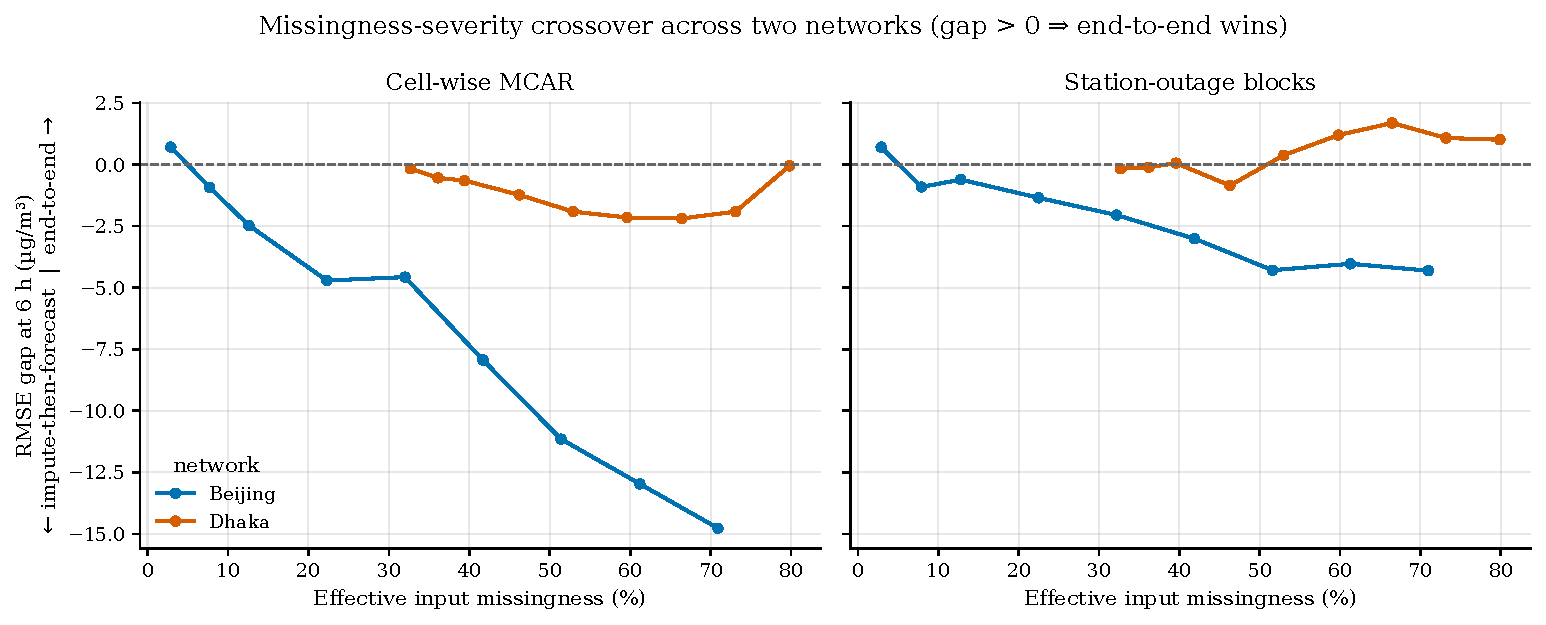
\includegraphics[width=\linewidth]{crossover_combined.pdf}
\caption{End-to-end advantage (best impute-then-forecast minus best end-to-end
RMSE; gap $>0\Rightarrow$ end-to-end wins) vs effective input missingness at
\SI{6}{\hour}. Under station outages the two networks diverge: on Dhaka the
advantage rises with severity and crosses zero ($\approx\!38\%$), while on the
highly periodic Beijing network the deep imputer stays ahead and its margin
grows. The choice depends on series imputability, not severity alone.}
\label{fig:crossover}
\end{figure}

\begin{table}[t]
\centering
\caption{Decision rule from the crossover study: effective input missingness at
which end-to-end overtakes impute-then-forecast, per mechanism and horizon
(\texttt{decision\_summary}). Values are filled from the regenerated table.}
\label{tab:decision}
\small
\begin{table}
\caption{Decision rule: effective input missingness at which end-to-end forecasting overtakes impute-then-forecast, per mechanism and horizon.}
\label{tab:decision}
\begin{tabular}{llll}
\toprule
 &  & crossover\_missing\_pct & recommendation \\
mode & horizon &  &  \\
\midrule
\multirow[t]{3}{*}{miss} & 6 & >max & impute-then-forecast at all tested severities \\
 & 24 & >max & impute-then-forecast at all tested severities \\
 & 72 & >max & impute-then-forecast at all tested severities \\
\cline{1-4}
\multirow[t]{3}{*}{out} & 6 & 38.4 & end-to-end above \textasciitilde 38.4\% input missingness \\
 & 24 & 70.8 & end-to-end above \textasciitilde 70.8\% input missingness \\
 & 72 & >max & impute-then-forecast at all tested severities \\
\cline{1-4}
\bottomrule
\end{tabular}
\end{table}

\end{table}

\subsection{Mechanism: the advantage tracks per-window incompleteness}
\label{sec:mechanism}

Figure~\ref{fig:stratified} stratifies clean-test windows by their input
missingness and plots the end-to-end-minus-two-stage RMSE gap per stratum. The
gap is near zero on the most complete windows and widens monotonically on the
most incomplete ones, showing that the aggregate parity hides a window-level
trade: the end-to-end model earns its keep exactly where the input is most
degraded.

\begin{figure}[t]
\centering

\includegraphics[width=0.8\linewidth]{stratified_gap.pdf}
\caption{Dhaka: end-to-end advantage by per-window input missingness. The gap
widens on the most incomplete windows---mechanistic evidence, not an aggregate.}
\label{fig:stratified}
\end{figure}

\subsection{High-pollution episodes}
\label{sec:episodes}

Restricting to the operationally important hours with observed \pmf{}~$>\SI{150}{\ugm}$
(Table~\ref{tab:episode}), the proposed + miss-dropout variant is best at
\SI{6}{\hour} (\SI{130.2}{\ugm}) and \SI{24}{\hour} (\SI{125.3}{\ugm})---the same
configuration that is most outage-robust---while PatchTST is worst.

\begin{table}[t]
\centering
\caption{Dhaka high-pollution-episode \pmf{} RMSE (\ugm), observed
\pmf{}~$>\SI{150}{\ugm}$ (818/1135/1136 targets), three-seed mean~$\pm$~std
(selected models).}
\label{tab:episode}
\small
\begin{tabular}{lccc}
\toprule
Model & \SI{6}{\hour} & \SI{24}{\hour} & \SI{72}{\hour} \\
\midrule
Two-stage (SAITS)       & 133.21\,$\pm$\,1.20 & 126.30\,$\pm$\,0.89 & 134.80\,$\pm$\,0.85 \\
Two-stage (KNN)         & 134.80\,$\pm$\,1.60 & 130.13\,$\pm$\,0.67 & 134.06\,$\pm$\,1.73 \\
Proposed (MAT)          & 133.61\,$\pm$\,1.52 & 127.91\,$\pm$\,0.84 & 134.18\,$\pm$\,1.90 \\
Proposed + miss-dropout & \textbf{130.17\,$\pm$\,3.65} & \textbf{125.29\,$\pm$\,2.49} & \textbf{133.00\,$\pm$\,2.73} \\
PatchTST                & 152.52\,$\pm$\,1.68 & 147.21\,$\pm$\,4.19 & 152.22\,$\pm$\,3.31 \\
\bottomrule
\end{tabular}
\end{table}

\subsection{Deployability}
\label{sec:efficiency}

The proposed model is \num{406}k parameters at \SI{1.8}{\milli\second} per window
with \emph{no} imputation stage. The two-stage pipelines carry an imputer that
must be refit and re-run on every data refresh: the SAITS imputer alone is
\SI{5.6}{\minute} to fit and is re-applied at inference. On equal accuracy, the
absence of a serving-time imputation stage is the practical advantage that
generalizes across both networks, independent of where the deployment sits
relative to the crossover.

% =====================================================================
\section{Discussion}
\label{sec:discussion}

Our results recast a question usually answered by a single benchmark number into
a conditional decision with two axes. End-to-end and impute-then-forecast are not
globally ranked; their ordering depends on missingness severity, its structure,
and---critically---the imputability of the series. Under the benign cell-wise
MCAR mechanism, a strong deep imputer is hard to beat on both networks. Under the
realistic station-outage mechanism, the ordering depends on whether the series is
imputable: on highly periodic data (Beijing) a deep imputer reconstructs even
long outage blocks and wins throughout, whereas on noisier, less periodic data
(Dhaka) imputation has little to exploit once outages are severe and end-to-end
forecasting overtakes past a within-network crossover. The practical
recommendation is therefore: characterize the deployment's effective missingness,
its structure, and how imputable its series are; in the high-missingness,
low-imputability regime forecast end-to-end (preferably with missingness dropout)
and drop the imputation stage; otherwise impute then forecast. Either way, the
end-to-end model's accuracy parity and absence of a serving-time imputation stage
make it a safe default to deploy and a cheap one to serve.

% =====================================================================
\section{Limitations}
\label{sec:limitations}

Both networks are air quality; the crossover's numerical location may differ in
other domains, though the qualitative mechanism (outages destroy the
cross-section) should transfer. Synthetic corruption is a proxy for additional
real missingness; we mitigate this by matching the corruption to the empirically
dominant outage mechanism. The architecture is intentionally simple and
per-station; spatial models may shift accuracy but are orthogonal to the
crossover question. Beijing models were trained on GPU and are not bit-identical
to CPU runs at the same seed.

% =====================================================================
\section{Conclusion}
\label{sec:conclusion}

We characterized when to forecast air quality end-to-end rather than
impute-then-forecast, showing the choice turns on missingness severity, its
structure, and series imputability rather than any single threshold: on the
severely incomplete, less-structured Dhaka network end-to-end forecasting
overtakes a deep imputer past a within-network crossover, while on the highly
periodic Beijing network the imputer wins throughout. A deliberately simple,
CPU-deployable missingness-aware Transformer reaches accuracy parity with strong
pipelines---including a quality-gated deep imputer and the missingness-native
GRU-D---and, with missingness dropout, degrades most gracefully in the severe
regime and on high-pollution episodes. The contribution is a deployment
decision rule, a reproducible multi-seed benchmark, and the reminder that
unhandled sensor error codes can silently distort every reported number.

\paragraph{Reproducibility.}
The pipeline is config-driven and deterministic; all tables and figures
regenerate from a single command, every learned model is trained with three
seeds, and 86 unit tests cover the data, model, and evaluation contracts.

\bibliographystyle{elsarticle-num}
\bibliography{references}

\end{document}
